\chapter{概率生成模型}
\label{chap:pgm-generative}

给一张图像赋予概率，与从随机数生成一张图像，是同一个模型的两种用法，却不一定具有相同的计算难度。一个网络可以迅速生成样本，但无法回答某个给定样本的密度；另一个模型可以精确计算完整观测的似然，却需要许多顺序步骤才能生成新样本。前文的图分解、边缘化和近似推断，正好提供了区分这些情况的工具：需要计算的概率是什么，哪些变量尚未观测，困难又落在哪个求和、积分或变换上？

本章围绕三个相互关联的问题展开：复杂的观测分布怎样保持归一化，训练时实际优化的量与似然是什么关系，生成一个新样本需要付出什么代价。潜变量边缘化、可逆变量变换和人工随机过程分别给出一种答案。三者都可以使用神经网络，但网络在其中承担的概率角色不同。理解这些角色，比把生成模型视为网络名称的列表更能帮助我们判断它们的能力与边界。

\section{概率生成模型的共同问题}
\label{sec:pgm-generative-common}

设训练样本$\bm{x}_1,\ldots,\bm{x}_n$独立同分布地来自未知分布$p_{\mathrm{data}}$，希望用参数向量$\bm{\theta}$确定的$p_{\bm{\theta}}$近似它。除特别说明外，本章讨论$\bm{x}\in\mathbb{R}^{d}$上的连续密度，概率都是对区域积分得到的；密度在一个点上可以大于$1$。二值或离散观测使用概率质量函数，不能把连续密度值直接当成某个像素取值的概率。

\term{概率生成模型}（probabilistic generative model）为可能出现的观测规定一个分布，并据此生成新观测。对显式密度模型，归一化要求$\int p_{\bm{\theta}}(\bm{x})\,\mathrm{d}\bm{x}=1$。最大似然学习最小化
\begin{equation}
  \label{eq:pgm-generative-nll}
  J(\bm{\theta})
  =-\frac{1}{n}\sum_{i=1}^{n}\log p_{\bm{\theta}}(\bm{x}_i).
\end{equation}
这个表达式很短，但它没有说明每个对数密度如何计算。若模型含有潜变量，边缘化可能使似然难以求值；若只提供一个从噪声到数据的程序，则分布虽然存在，也未必有可计算的密度。训练、密度评价、采样和潜变量推断因此需要分别说明。

第~\ref{sec:pgm-static-directed-autoregressive}节的自回归模型提供了一个基线：用已归一化的一维条件分布按链式法则构成联合分布，完整观测的似然可精确评价，通常的祖先采样则要按给定顺序生成各个分量。本章不重复其网络参数化。下面比较的三种机制把困难放在别处：VAE对一个联合分布中的潜变量积分；规范化流通过双射追踪体积变化；扩散模型把生成拆成许多局部随机转移。

这不是对生成模型的穷尽分类，也不是三种新的条件独立性图语义。VAE直接使用有向潜变量图；离散扩散可以写成沿人工噪声索引展开的有向Markov链；规范化流的密度则来自确定性双射和变量变换公式。一个双射的计算图不自动具有有向图模型的条件独立性含义。后文还会用概率电路作补充比较：除了放宽函数形式，也可以限制计算结构，换取精确的边缘化和条件查询。

为使三种机制可直接核对，本章反复使用人为构造的一维目标$X\sim\mathcal{N}(0,5)$。它可以由两个独立高斯变量相加得到，也可以由标准高斯缩放得到，还可以作为前向扩散的起点。这个例子没有复杂数据的表达难题，却能把分布、密度和随机路径之间的区别算清楚。

\section{变分自编码器}
\label{sec:pgm-generative-vae}

\subsection{有向潜变量模型}
\label{sec:pgm-generative-latent-model}

如果观测中的相关变化由少量未观测因素共同引起，可以先生成这些因素，再生成观测。\term{变分自编码器}（variational autoencoder, VAE）将这种有向潜变量模型与可学习的近似后验结合起来：生成网络规定潜变量怎样产生观测，推断网络则根据观测估计哪些潜变量较为可能。它不是仅仅把输入压缩后还原的确定性自编码器\scite{kingma2013}

令$\bm{z}\in\mathbb{R}^{k}$，通常取先验$p(\bm{z})=\mathcal{N}(\bm{0},\bm{I}_k)$，再用神经网络输出条件分布$p_{\bm{\theta}}(\bm{x}\mid\bm{z})$的参数。生成联合分布与观测边缘分布为
\begin{equation}
  \label{eq:pgm-generative-vae-joint}
  \begin{aligned}
    p_{\bm{\theta}}(\bm{x},\bm{z})
      &=p(\bm{z})p_{\bm{\theta}}(\bm{x}\mid\bm{z}),\\
    p_{\bm{\theta}}(\bm{x})
      &=\int p(\bm{z})p_{\bm{\theta}}(\bm{x}\mid\bm{z})
          \,\mathrm{d}\bm{z}.
  \end{aligned}
\end{equation}
只要先验和每个条件分布都归一化，非负积分交换便说明观测分布也归一化。难点不是证明积分等于$1$，而是对某个$\bm{x}$计算这个积分的数值。

以连续观测为例，\term{解码器}（decoder）不是直接输出唯一的$\bm{x}$，而是输出观测分布的参数。一个常用设定是
\begin{equation}
  \label{eq:pgm-generative-gaussian-decoder}
  p_{\bm{\theta}}(\bm{x}\mid\bm{z})
  =\mathcal{N}\bigl(\bm{x};
    \bm{g}_{\bm{\theta}}(\bm{z}),\tau^2\bm{I}_d\bigr),
  \qquad \tau>0.
\end{equation}
其中$\bm{g}_{\bm{\theta}}:\mathbb{R}^{k}\to\mathbb{R}^{d}$给出条件均值，$\tau^2$给出条件噪声方差。生成时先抽取$\bm{z}\sim p$，再抽取独立的$\bm{\eta}\sim\mathcal{N}(\bm{0},\bm{I}_d)$，返回$\bm{x}=\bm{g}_{\bm{\theta}}(\bm{z})+\tau\bm{\eta}$。只显示$\bm{g}_{\bm{\theta}}(\bm{z})$相当于显示条件均值，不是从式~\eqref{eq:pgm-generative-gaussian-decoder}完整采样。

在线性情形$\bm{g}_{\bm{\theta}}(\bm{z})=\bm{W}\bm{z}+\bm{b}$，其中$\bm{W}\in\mathbb{R}^{d\times k}$，便回到第~\ref{sec:pgm-static-directed-linear-gaussian}节的各向同性噪声模型。这里用$k$表示潜变量维数、$\tau^2$表示噪声方差，边缘分布仍然是高斯：
\[
  p_{\bm{\theta}}(\bm{x})
  =\mathcal{N}\bigl(\bm{x};
    \bm{b},\bm{W}\bm{W}^{\top}+\tau^2\bm{I}_d\bigr).
\]
后验也能由配平方得到。把对数联合分布中与$\bm{z}$有关的二次项合并，后验精度矩阵为$\bm{I}_k+\tau^{-2}\bm{W}^{\top}\bm{W}$，因而
\begin{equation}
  \label{eq:pgm-generative-linear-posterior}
  \begin{aligned}
    \bm{\Sigma}
      &=\bigl(\bm{I}_k+\tau^{-2}\bm{W}^{\top}\bm{W}\bigr)^{-1},\\
    \bm{m}(\bm{x})
      &=\tau^{-2}\bm{\Sigma}\bm{W}^{\top}(\bm{x}-\bm{b}),\\
    p_{\bm{\theta}}(\bm{z}\mid\bm{x})
      &=\mathcal{N}\bigl(\bm{z};\bm{m}(\bm{x}),\bm{\Sigma}\bigr).
  \end{aligned}
\end{equation}
非线性解码器可以产生弯曲、非高斯的观测分布，但$\lVert\bm{x}-\bm{g}_{\bm{\theta}}(\bm{z})\rVert_2^2$通常不再是$\bm{z}$的二次式，解析边缘化与高斯后验随之消失。VAE使用前文的近似推断处理这一计算困难，并没有改变式~\eqref{eq:pgm-generative-vae-joint}的概率定义。

\begin{example}[同一观测分布的潜变量解释]
  \label{ex:pgm-generative-gaussian-latent}
  取$Z\sim\mathcal{N}(0,1)$、$E\sim\mathcal{N}(0,1)$且二者独立，令$X=2Z+E$，于是$X\sim\mathcal{N}(0,5)$。观测$x=2$后，
  \[
    p(z\mid x=2)\propto
    \exp\left[-\frac{1}{2}\{z^2+(2-2z)^2\}\right]
    \propto\exp\left[-\frac{5}{2}(z-0.8)^2\right].
  \]
  后验因此为$\mathcal{N}(0.8,0.2)$。虽然$x$已知，$z$仍不唯一，因为观测还混入了独立噪声。这个不确定性将与Flow中唯一的逆像形成对照。
\end{example}

\subsection{VAE目标与摊销后验}
\label{sec:pgm-generative-vae-objective}

式~\eqref{eq:pgm-variational-elbo}已经给出一般ELBO，第~\ref{sec:pgm-variational-amortized}节说明了摊销推断和重参数化梯度。将联合分布~\eqref{eq:pgm-generative-vae-joint}代入，单个观测的证据下界具体成为
\begin{equation}
  \label{eq:pgm-generative-vae-elbo}
  \begin{aligned}
    \mathcal{L}(\bm{\theta},\bm{\phi};\bm{x})
    ={}&\mathbb{E}_{q_{\bm{\phi}}(\bm{z}\mid\bm{x})}
       [\log p_{\bm{\theta}}(\bm{x}\mid\bm{z})]\\
      &-\operatorname{KL}\bigl(
       q_{\bm{\phi}}(\bm{z}\mid\bm{x})\,\|\,p(\bm{z})\bigr)
      \leq\log p_{\bm{\theta}}(\bm{x}).
  \end{aligned}
\end{equation}
\term{编码器}（encoder）给出的是$q_{\bm{\phi}}(\bm{z}\mid\bm{x})$的分布参数，而不是生成模型中一条额外的反向边。本章按VAE惯例用$\bm{\phi}$统称共享编码器的权重，对应第~\ref{sec:pgm-variational-amortized}节的$\bm{\omega}$；随观测变化的均值、尺度是网络输出，不是各样本分别训练的权重。模型参数$\bm{\theta}$则属于生成分布。图~\ref{fig:pgm-generative-vae}把两套计算分开：观测从先验和解码器生成，编码器只服务于训练及观测后的近似推断。把两种箭头叠成一个有向环，会混淆生成联合分布与推断程序。

\begin{figure}[htbp]
  \centering
  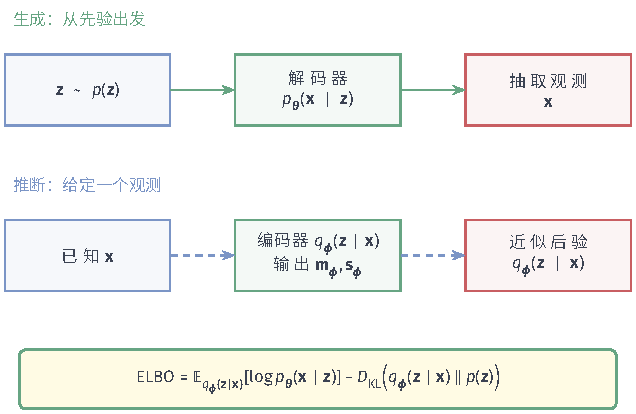
\includegraphics[width=\linewidth]{figures/03-models/03-probabilistic-graphical-models/tikz/pgm-generative-vae/figure.pdf}
  \caption{VAE的生成与推断分工。上行实线表示先抽潜变量、再按$p_{\bm\theta}(\bm x\mid\bm z)$抽观测的生成顺序；下行虚线表示用$q_{\bm\phi}(\bm z\mid\bm x)$构造近似后验的推断顺序。编码器与解码器框内直接写出概率对象，底部公式带给出连接两条路径的ELBO；两行不合并成同一个有向图。}
  \label{fig:pgm-generative-vae}
\end{figure}

常用编码器取对角高斯
\[
  q_{\bm{\phi}}(\bm{z}\mid\bm{x})
  =\mathcal{N}\!\left(
    \bm{z};\bm{m}_{\bm{\phi}}(\bm{x}),
    \operatorname{diag}\bigl(\bm{s}_{\bm{\phi}}^2(\bm{x})\bigr)
    \right),
\]
其中每个$s_{\bm{\phi},j}(\bm{x})>0$。网络可以输出对数方差以保证正性。对标准高斯先验，KL项解析可得：
\begin{equation}
  \label{eq:pgm-generative-diagonal-kl}
  \operatorname{KL}(q_{\bm{\phi}}\,\|\,p)
  =\frac{1}{2}\sum_{j=1}^{k}
     \bigl(m_{\bm{\phi},j}^2+s_{\bm{\phi},j}^2
            -1-\log s_{\bm{\phi},j}^2\bigr).
\end{equation}
这里省略了各分量对$\bm{x}$的依赖。期望项用$\bm{z}=\bm{m}_{\bm{\phi}}(\bm{x})+\bm{s}_{\bm{\phi}}(\bm{x})\odot\bm{\epsilon}$估计，其中$\bm{\epsilon}\sim\mathcal{N}(\bm{0},\bm{I}_k)$，$\odot$表示逐元素乘法。如此便可沿第~\ref{chap:pgm-variational}章的路径导数对两组网络参数求梯度，无须对每个样本另解一个完整优化问题。

图~\ref{fig:vae-reparameterization-training}将噪声抽样与参数相关的可微变换分开。独立噪声不依赖编码器参数，梯度通过均值、尺度与解码器传回；生成时则从先验进入解码器。

\begin{figure*}[htbp]
  \centering
  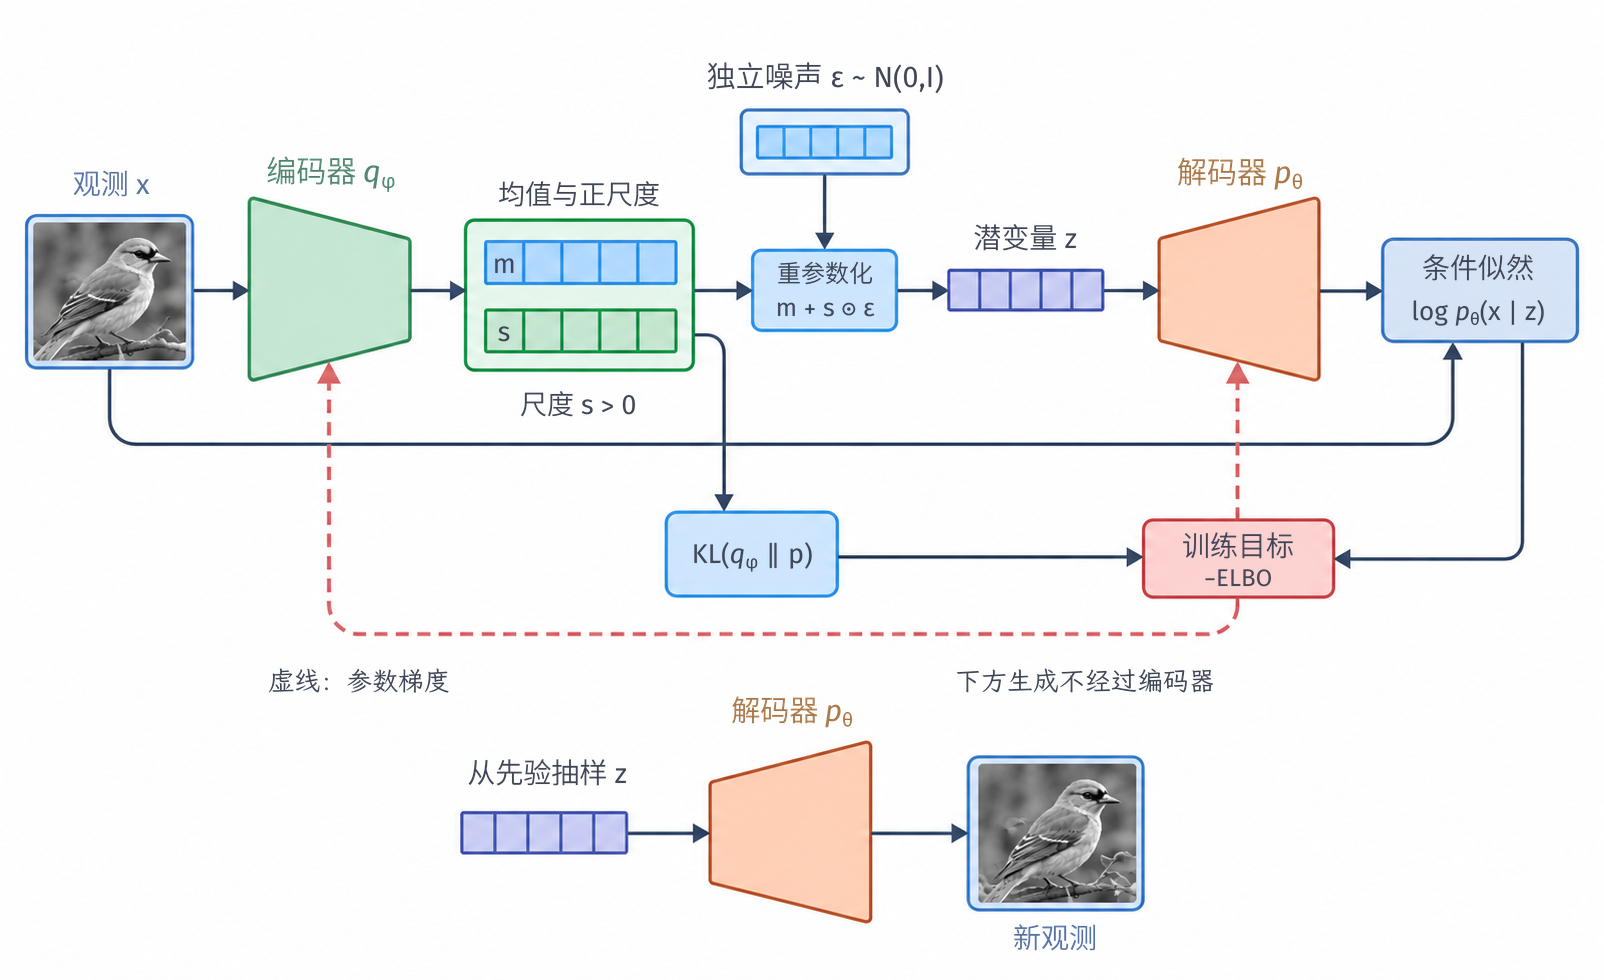
\includegraphics[width=\linewidth]{figures/03-models/03-probabilistic-graphical-models/generated/vae-reparameterization-training/figure.png}
  \caption{对角高斯VAE的重参数化与训练。编码器给出均值$\bm m$和正尺度$\bm s$，独立标准正态噪声经$\bm z=\bm m+\bm s\odot\bm\epsilon$形成潜变量，并进入解码器规定的条件分布。重构对数似然的期望与KL项组成ELBO，图中的负ELBO框表示训练目标。生成阶段从先验抽样，不经过编码器；鸟图为概念插画。}
  \label{fig:vae-reparameterization-training}
\end{figure*}

所谓“重构项”是条件对数似然，不是与分布无关的距离。式~\eqref{eq:pgm-generative-gaussian-decoder}给出
\begin{equation}
  \label{eq:pgm-generative-reconstruction}
  -\log p_{\bm{\theta}}(\bm{x}\mid\bm{z})
  =\frac{\lVert\bm{x}-\bm{g}_{\bm{\theta}}(\bm{z})\rVert_2^2}
          {2\tau^2}
    +\frac{d}{2}\log(2\pi\tau^2).
\end{equation}
只有固定$\tau$时，最后一项才是训练常数。学习方差时把对数方差项删掉，会得到另一个目标，并可能让模型仅靠扩大方差减少平方误差的权重。对于二值观测$x_j\in\{0,1\}$，若解码器输出独立Bernoulli参数$\pi_j(\bm{z})$，负对数似然则为
\[
  -\sum_{j=1}^{d}
    \bigl[x_j\log\pi_j(\bm{z})
      +(1-x_j)\log(1-\pi_j(\bm{z}))\bigr].
\]
这解释了交叉熵的来源。连续灰度值即使落在$[0,1]$，也不是Bernoulli随机变量的取值；直接套用这个损失需要另行说明其代理目标含义。离散像素可以用类别质量函数，或对连续条件密度在量化区间内积分。

在例~\ref{ex:pgm-generative-gaussian-latent}中，让编码器恰好输出$q(z\mid2)=\mathcal{N}(0.8,0.2)$，可以逐项复核ELBO：
\[
  \begin{aligned}
    \mathbb{E}_{q}(2-2Z)^2&=(2-1.6)^2+4(0.2)=0.96,\\
    \mathbb{E}_{q}\log p(2\mid Z)&=-\tfrac12\log(2\pi)-0.48,\\
    \operatorname{KL}(q\,\|\,p)&=
       \tfrac12\bigl(0.8^2+0.2-1-\log0.2\bigr).
  \end{aligned}
\]
合计$\mathcal{L}\approx-2.12366$，与$\log\mathcal{N}(2;0,5)=-\tfrac12\log(10\pi)-0.4$相等。若编码器忽略$x$而总输出先验，ELBO降为$-\tfrac12\log(2\pi)-4\approx-4.91894$。观测模型没有改变，下界变松来自推断分布没有跟上后验。

实际训练从一个小批量中取观测，编码器输出分布参数，为每个观测抽少量标准噪声，用式~\eqref{eq:pgm-generative-vae-elbo}的随机估计更新$\bm{\theta}$和$\bm{\phi}$，反复遍历数据直至达到预算或验证指标停止改善。若一次编码和一次解码的代价分别为$C_{\mathrm{enc}}$和$C_{\mathrm{dec}}$，每个观测使用一个潜变量样本时，前向计算约为$O(C_{\mathrm{enc}}+C_{\mathrm{dec}}+k)$，反向传播通常为同阶；使用更多样本降低部分蒙特卡洛方差，但增加解码成本。无条件生成不需要编码器，观测后的快速近似推断则只运行编码器。

理解失败原因还要区分三个层次。\term{模型近似误差}（model approximation error）来自候选$p_{\bm{\theta}}$本身不能充分表示数据分布；即使精确求解最大似然目标也不能消除它。固定模型参数后，限制近似后验的形状会造成\term{近似族误差}（variational approximation error）；同一族中，每个观测各自可选的最优参数又未必能由一个共享编码器同时给出，这部分是\term{摊销误差}（amortization error）。具体地，设$\mathcal{Q}$为候选后验族，记$\mathcal{L}_{\mathcal{Q}}^*(\bm{x})=\sup_{q\in\mathcal{Q}}\mathcal{L}(\bm{\theta},q;\bm{x})$，且$q_{\bm{\phi}}(\cdot\mid\bm{x})\in\mathcal{Q}$，则
\begin{equation}
  \label{eq:pgm-generative-inference-gaps}
  \begin{aligned}
    \log p_{\bm{\theta}}(\bm{x})
      -\mathcal{L}(\bm{\theta},\bm{\phi};\bm{x})
    ={}&\bigl[\log p_{\bm{\theta}}(\bm{x})
             -\mathcal{L}_{\mathcal{Q}}^*(\bm{x})\bigr]\\
       &+\bigl[\mathcal{L}_{\mathcal{Q}}^*(\bm{x})
             -\mathcal{L}(\bm{\theta},\bm{\phi};\bm{x})\bigr].
  \end{aligned}
\end{equation}
两项都非负。后一项对实际训练出的编码器还包含优化不足；只有像式~\eqref{eq:pgm-variational-amortization-gap}那样进一步比较最优共享编码器，才能把纯粹的摊销限制与优化误差分开。增加解码器容量、扩大后验族、改进编码器优化，分别作用于不同问题，不能彼此替代。

\subsection{生成能力与失效模式}
\label{sec:pgm-generative-vae-failure}

潜变量维度$k$影响模型把哪些变化交给$\bm{z}$表示，但$k<d$并不意味着观测必然没有$d$维密度。只要式~\eqref{eq:pgm-generative-gaussian-decoder}中的$\tau>0$，条件噪声就覆盖全部观测维度。若把噪声去掉，光滑低维解码器的输出才通常集中在低维集合上。增大$k$可以减轻表示瓶颈，也会增加需要学习和推断的自由度；它不保证所有潜变量都被使用。

当给定潜变量后仍有多种明显不同的观测可能，固定方差的单一高斯条件似然按平方误差拟合其均值。
\BookTheoremRef{thm:probability-conditional-mean-l2-projection}{第一卷“数学准备”的条件均值最小平方误差定理}
因而给出总体最优均值$\mathbb E[\bm X\mid\bm z]$，逐坐标应用时要求有限二阶矩。
例如边缘等概率出现在左右两处，均值图像会保留两处较淡的边缘。
这是模糊重构的一种机制；更有表达力的条件似然可表示多种结果，
从简单高斯额外抽噪声却不能自动恢复缺少的结构。

另一种失败是编码几乎不再携带观测信息。本节用\term{后验坍塌}（posterior collapse）指编码器的近似后验接近先验，即$q_{\bm{\phi}}(\bm{z}\mid\bm{x})\approx p(\bm{z})$；若只有部分坐标出现这种现象，则这些坐标对应的近似后验不再明显依赖观测。这一口径描述的是$q_{\bm{\phi}}$，不能直接据此判断生成模型的真实后验$p_{\bm{\theta}}(\bm{z}\mid\bm{x})$。前面的高斯例子已经给出对照：固定例~\ref{ex:pgm-generative-gaussian-latent}的生成模型，让编码器总输出先验，在$x=2$时真实后验仍为$\mathcal{N}(0.8,0.2)$，只是近似推断没有跟上它。

若解码器本身忽略全部潜变量，即$p_{\bm{\theta}}(\bm{x}\mid\bm{z})=p_{\bm{\theta}}(\bm{x})$，则真实后验也等于先验$p(\bm{z})$。固定这一生成模型时，ELBO在$q_{\bm{\phi}}(\bm{z}\mid\bm{x})=p(\bm{z})$处达到最大。强大的解码器若能绕过潜变量解释数据，减少KL代价可能比利用潜变量更有利；优化过程也可能让模型过早进入这一状态。因此，编码器的$\operatorname{KL}(q_{\bm{\phi}}\,\|\,p)$接近零可以作为坍塌线索，但不能单独证明解码器已忽略潜变量；它也不意味着所有生成能力都丧失了，因为解码器本身仍可能生成数据。

编码器在训练数据上使用的潜空间，与无条件生成时抽取的先验空间，也未必完全一致。定义\term{聚合后验}（aggregated posterior）
\begin{equation}
  \label{eq:pgm-generative-aggregated-posterior}
  q_{\mathrm{agg}}(\bm{z})
  =\mathbb{E}_{\bm{X}\sim p_{\mathrm{data}}}
       [q_{\bm{\phi}}(\bm{z}\mid\bm{X})],
\end{equation}
即把不同观测的编码分布按数据频率混合。假设相关KL有限，在$\log(q_{\bm{\phi}}/p)$中加减$\log q_{\mathrm{agg}}$，可得
\begin{equation}
  \label{eq:pgm-generative-kl-information}
  \mathbb{E}_{p_{\mathrm{data}}}
    \operatorname{KL}(q_{\bm{\phi}}(\bm{z}\mid\bm{X})\,\|\,p(\bm{z}))
  =I_q(\bm{X};\bm{Z})+
    \operatorname{KL}(q_{\mathrm{agg}}\,\|\,p).
\end{equation}
其中$I_q$是联合分布$p_{\mathrm{data}}(\bm{x})q_{\bm{\phi}}(\bm{z}\mid\bm{x})$下的互信息。第一部分惩罚编码携带的数据信息，第二部分惩罚聚合后验偏离先验。因此，逐样本KL既不只是“让潜空间像高斯”，也不保证有限训练后两者完全相同。若先验在编码器很少访问的区域仍有明显质量，生成时就可能进入解码器缺少训练支持的区域。

常见修正应按改变的对象理解。把KL系数从小值逐渐提高到$1$，改变的是训练路径；若最终保持$\lambda\ne1$，优化的$\mathbb{E}_q\log p_{\bm{\theta}}(\bm{x}\mid\bm{z})-\lambda \operatorname{KL}(q\,\|\,p)$就不再是原始ELBO。$\lambda\geq1$时它仍不大于原ELBO，$\lambda<1$时则没有相同的下界保证。限制解码器绕过潜变量的信息通路改变模型结构；使用更灵活的后验主要缩小推断差距；学习一个可评价密度的先验则改变生成模型及KL比较的对象。这些措施不提供无条件的防坍塌保证。

已有标签或其他条件$\bm{c}$时，\term{条件VAE}（conditional VAE）把“要生成哪一类观测”直接交给模型，使用$p_{\bm{\theta}}(\bm{z}\mid\bm{c})p_{\bm{\theta}}(\bm{x}\mid\bm{z},\bm{c})$以及$q_{\bm{\phi}}(\bm{z}\mid\bm{x},\bm{c})$。这时潜变量只需解释给定$\bm{c}$之后剩余的变化。\term{层次VAE}（hierarchical VAE）则设置多层随机潜变量，例如$p(\bm{z}_2)p_{\bm{\theta}}(\bm{z}_1\mid\bm{z}_2)p_{\bm{\theta}}(\bm{x}\mid\bm{z}_1)$，让不同层分担不同依赖。它增加了模型的随机结构，同时也增加了后验的耦合；不是在确定性解码网络中多加几层就自动得到层次VAE。

\section{基于可逆变换的密度模型}
\label{sec:pgm-generative-flows}

\subsection{变量变换与精确密度}
\label{sec:pgm-generative-change-of-variables}

VAE的积分困难来自同一个观测可以由许多潜变量和观测噪声共同产生。如果让每个观测恰好对应一个基础变量，就可以用体积变化取代边缘化。\term{规范化流}（normalizing flow, Flow）把一个可评价密度的基础分布经过一串可逆变换推送到数据空间，并在变换中追踪密度。这里沿用第~\ref{chap:pgm-overview}章的“规范化流”译名；文献也常称其为归一化流\scite{pgm-generative-papamakarios2021}

设$\bm Z\sim p_0$，$\bm X=f_{\bm\theta}(\bm Z)$，基础变量与观测均为$d$维。
沿用\BookSectionRef{sec:analysis-coordinate-change-integral-applications}{第一卷“数学准备”的积分变量变换小节}
和\BookSectionRef{sec:rv-pushforward}{第一卷“数学准备”的分布推送小节}，
在开集间的连续可微双射、连续可微逆及非零Jacobian行列式条件下，
当前流模型的密度为
\begin{equation}
  \label{eq:pgm-generative-flow-density}
  \begin{aligned}
    p_{\bm{\theta}}(\bm{x})
      &=p_0(f_{\bm{\theta}}^{-1}(\bm{x}))
         \left|\det\bm{J}_{f_{\bm{\theta}}^{-1}}(\bm{x})\right|,\\
    \log p_{\bm{\theta}}(\bm{x})
      &=\log p_0(\bm{z})-
         \log\left|\det\bm{J}_{f_{\bm{\theta}}}(\bm{z})\right|.
  \end{aligned}
\end{equation}
这里$\bm z=f_{\bm\theta}^{-1}(\bm x)$，$\bm J_f$为卷一约定的Jacobian矩阵。
行列式修正保留变换前后的概率质量，因此无需另估配分函数。
分段光滑网络仍须核验变量变换条件；仅有几乎处处可微和双射不足以保证此密度公式。

若$f=f_K\circ\cdots\circ f_1$，令$\bm{h}_0=\bm{z}$、$\bm{h}_{\ell}=f_{\ell}(\bm{h}_{\ell-1})$、$\bm{h}_K=\bm{x}$，链式法则给出
\begin{equation}
  \label{eq:pgm-generative-flow-composition}
  \log p_{\bm{\theta}}(\bm{x})
  =\log p_0(\bm{h}_0)
   -\sum_{\ell=1}^{K}
      \log|\det\bm{J}_{f_{\ell}}(\bm{h}_{\ell-1})|.
\end{equation}
训练时从数据逆行到基础变量，累积每层对数行列式，再对式~\eqref{eq:pgm-generative-nll}求梯度；生成时从$p_0$抽样并正向通过各层。这些计算不含变分下界。但数学上存在逆函数，不等于逆函数计算便宜；一般稠密$d\times d$矩阵用常规分解计算行列式要$O(d^3)$运算，形成完整Jacobian本身也可能昂贵。可用的流结构必须同时控制逆变换和体积因子的成本。

\begin{example}[用缩放得到相同的一维密度]
  \label{ex:pgm-generative-gaussian-flow}
  取$Z\sim\mathcal{N}(0,1)$，令$X=\sqrt{5}Z$，同样得到$\mathcal{N}(0,5)$。给定$x=2$，唯一逆像是$z=2/\sqrt5$，因此
  \[
    \log p(2)=-\tfrac12\log(2\pi)
              -\tfrac12(2/\sqrt5)^2-\log\sqrt5
             \approx-2.12366.
  \]
  这与VAE例子的观测密度相同，但这里没有$\mathcal{N}(0.8,0.2)$那样的潜变量后验不确定性。两个生成机制可以定义同一个观测分布，观测似然无法单独识别哪个潜变量解释才是实际原因。
\end{example}

标准Flow要求基础空间与观测空间同维，因为上述Jacobian必须是同维变换的方阵。重排、分块输出和保留旁路变量可以改变中间张量形状，却没有丢弃总自由度。若真地丢弃一些坐标，就要对它们边缘化；若增加随机变量，则要说明扩展空间的联合密度。连续Flow处理离散观测也需要桥接：以单位宽度量化为例，对量化值$\bm{y}$，离散质量是$p(\bm{y})=\int_{[0,1)^d}p_{\mathrm{cont}}(\bm{y}+\bm{u})\,\mathrm{d}\bm{u}$，不是$p_{\mathrm{cont}}(\bm{y})$。取$\bm{U}$在$[0,1)^d$上均匀分布，均匀去量化的$\mathbb{E}_{\bm{U}}\log p_{\mathrm{cont}}(\bm{y}+\bm{U})$由Jensen不等式给出该对数质量的下界；若还有缩放预处理，必须计入其Jacobian。

\subsection{可逆网络结构}
\label{sec:pgm-generative-invertible-networks}

让每层都具有容易计算的Jacobian，可以在可逆性与非线性之间取得实际可用的折中。\term{仿射耦合层}（affine coupling layer）把坐标分成两个非空、不相交的块$A,B$，保留一块，用它决定另一块的缩放和平移：
\begin{equation}
  \label{eq:pgm-generative-coupling}
  \begin{aligned}
    \bm{x}_A&=\bm{z}_A,\\
    \bm{x}_B&=\bm{z}_B\odot
       \exp\bigl(\bm{a}_{\bm{\theta}}(\bm{z}_A)\bigr)
          +\bm{b}_{\bm{\theta}}(\bm{z}_A).
  \end{aligned}
\end{equation}
指数逐元素作用，保证每个缩放因子为正。给定$\bm{x}$，先恢复$\bm{z}_A=\bm{x}_A$，再计算$\bm{z}_B=(\bm{x}_B-\bm{b}_{\bm{\theta}}(\bm{x}_A))\odot\exp(-\bm{a}_{\bm{\theta}}(\bm{x}_A))$。两个子网络本身都不要求可逆，因为它们的输入已经由保留块确定。Real NVP以这类耦合变换构造密度模型\scite{pgm-generative-dinh2017}

按$A,B$的顺序排列坐标，Jacobian为
\begin{equation}
  \label{eq:pgm-generative-coupling-jacobian}
  \begin{aligned}
    \bm{J}_{f}
      &=
        \begin{pmatrix}
          \bm{I}&\bm{0}\\
          *&\operatorname{diag}(\exp\bm{a}_{\bm{\theta}}(\bm{z}_A))
        \end{pmatrix},\\
    \log|\det\bm{J}_{f}|
      &=\sum_{j=1}^{|B|}a_{\bm{\theta},j}(\bm{z}_A).
  \end{aligned}
\end{equation}
星号块包含复杂导数，但三角矩阵的行列式不需要它。图~\ref{fig:pgm-generative-coupling}展示了这种安排为何能兼顾灵活子网络与简单逆变换。单层始终不改变$A$块，表达能力有限；多层之间交换分块或插入可逆混合，才让不同坐标相互影响。若单层子网络代价为$C$，计算行列式的额外代价仅为$O(d)$，$K$层正向或逆向计算约需$O(K(C+d))$，这里不把子网络计算本身错误地算成线性成本。

\begin{figure}[htbp]
  \centering
  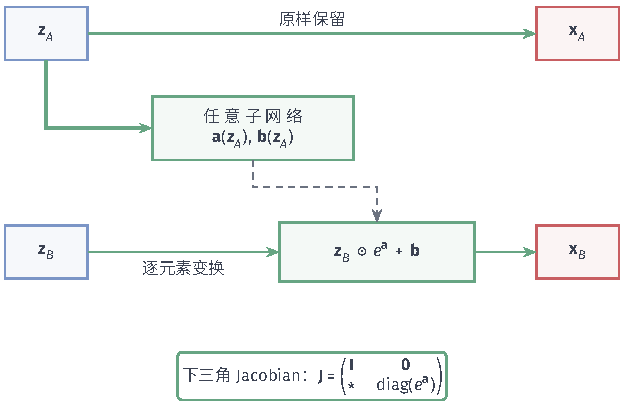
\includegraphics[width=\linewidth]{figures/03-models/03-probabilistic-graphical-models/tikz/pgm-generative-coupling/figure.pdf}
  \caption{仿射耦合层的计算依赖。粗线把$\bm z_A$送入任意子网络，该子网络只产生缩放和平移参数；下方逐元素仿射变换才真正改变$\bm z_B$。Jacobian为下三角结构，因此子网络不必可逆，整层的对数行列式只需对缩放对数求和。逆向计算先恢复原样保留的$\bm z_A$，再撤销缩放和平移。}
  \label{fig:pgm-generative-coupling}
\end{figure}

一个可复核的二维例子是$x_1=z_1$、$x_2=2z_2+z_1^2$。在$\bm{z}=(1,-1)$处，$\bm{x}=(1,-1)$，逆变换给出$z_2=(x_2-x_1^2)/2=-1$。Jacobian为$\left(\begin{smallmatrix}1&0\\2z_1&2\end{smallmatrix}\right)$，行列式恒为$2$。若基础分布为二维标准高斯，则该观测的对数密度为$-\log(2\pi)-1-\log2$；非线性的$z_1^2$改变坐标关系，却没有增加行列式的计算难度。

三角结构也可以逐坐标建立。\term{自回归流}（autoregressive flow）利用前面的坐标决定当前的可逆变换。这里讨论的是变换方向的计算取舍，不重述第~\ref{chap:pgm-static-directed}章的自回归建模。\term{掩码自回归流}（masked autoregressive flow, MAF）的一种形式为
\[
  x_j=\mu_j(\bm{x}_{<j})+
       \exp(a_j(\bm{x}_{<j}))z_j,\qquad j=1,\ldots,d,
\]
其中$\bm{x}_{<j}=(x_1,\ldots,x_{j-1})$。评价给定$\bm{x}$时，所有条件输入已知，掩码网络可并行给出各$\mu_j,a_j$，从而恢复$\bm{z}$并求出三角Jacobian的行列式；生成时$\bm{x}_{<j}$尚未齐备，必须顺序恢复坐标。

\term{逆自回归流}（inverse autoregressive flow, IAF）则把上式参数改成$\mu_j(\bm{z}_{<j})$和$a_j(\bm{z}_{<j})$。抽好全部基础噪声后，可以并行计算输出及这些新样本的密度；但对任意外部$\bm{x}$求逆时，要逐坐标解出$\bm{z}$。所以“采样后顺便计算其密度”与“对任意指定点计算密度”是不同任务。MAF和IAF的方向取舍已在原始MAF论文中明确比较\scite{pgm-generative-papamakarios2017}

还可以把许多离散层换成连续变换。\term{连续规范化流}（continuous normalizing flow, CNF）用常微分方程
\[
  \frac{\mathrm{d}\bm{h}_u}{\mathrm{d}u}
    =\bm{v}_{\bm{\theta}}(\bm{h}_u,u),
  \qquad 0\leq u\leq1,
\]
定义从$\bm{h}_0=\bm{z}$到$\bm{h}_1=\bm{x}$的映射。这里$u$是变换参数，不是数据的真实时间。一个充分的正则设定是速度场对空间连续可微、具有足够的Lipschitz控制，并且解在整个区间正反两向都存在；唯一解使不同轨迹不能在同一$u$相交，从而定义可逆流。

记$\rho_u$为$\bm{h}_u$的密度。小步映射的Jacobian为$\bm{I}+\Delta u\,\bm{J}_{\bm{v}}+o(\Delta u)$，结合$\log\det(\bm{I}+\Delta u\,\bm{A})=\Delta u\,\operatorname{tr}\bm{A}+o(\Delta u)$，可从式~\eqref{eq:pgm-generative-flow-density}得到\term{瞬时变量变换公式}（instantaneous change of variables）：
\begin{equation}
  \label{eq:pgm-generative-instantaneous-change}
  \begin{aligned}
    \frac{\mathrm{d}}{\mathrm{d}u}
         \log\rho_u(\bm{h}_u)
       &=-\nabla_{\bm{h}}\!\cdot
          \bm{v}_{\bm{\theta}}(\bm{h}_u,u),\\
    \log p_{\bm{\theta}}(\bm{x})
       &=\log p_0(\bm{z})
         -\int_0^1\nabla_{\bm{h}}\!\cdot
           \bm{v}_{\bm{\theta}}(\bm{h}_u,u)\,\mathrm{d}u.
  \end{aligned}
\end{equation}
散度$\nabla\cdot\bm{v}=\sum_j\partial v_j/\partial h_j$就是Jacobian的迹，表示局部体积膨胀率。CNF因而不必把每个有限层的Jacobian限制为三角形，却要反复求解速度场与散度。

高维时，迹仍可能昂贵。若$\mathbb{E}\bm{r}=\bm{0}$且$\mathbb{E}\bm{r}\bm{r}^{\top}=\bm{I}$，则$\operatorname{tr}\bm{A}=\mathbb{E}_{\bm{r}}[\bm{r}^{\top}\bm{A}\bm{r}]$；自动微分可以通过向量与Jacobian的乘积估计它。FFJORD将这种随机迹估计用于连续流\scite{pgm-generative-grathwohl2018}

这个恒等式保证固定矩阵下的迹估计无偏，不意味着一次估计精确，也不消除数值求解误差。连续流的似然有精确的数学定义，程序返回的通常是积分和迹的数值近似；正向、逆向都需要求解器，成本取决于函数评价次数和场的数值性质。

\subsection{生成模型与变分后验}
\label{sec:pgm-generative-flow-roles}

规范化流不一定直接变换观测空间。作为独立生成模型，它变换$\bm{z}$得到$\bm{x}$，并通过式~\eqref{eq:pgm-generative-flow-density}计算观测密度。作为VAE的近似后验，它变换一个给定$\bm{x}$的简单潜变量分布，得到更复杂的$q_{\bm{\phi}}(\bm{z}\mid\bm{x})$。后者改变的是推断族，生成联合分布$p_{\bm{\theta}}(\bm{x},\bm{z})$可以保持原样\scite{pgm-overview-rezende2015}

具体地，先抽$\bm{u}\sim q_0(\bm{u}\mid\bm{x})$，再令$\bm{z}=f_{\bm{\phi}}(\bm{u};\bm{x})$。只要求固定$\bm{x}$时对$\bm{u}$为合适的双射，就有
\begin{equation}
  \label{eq:pgm-generative-flow-posterior}
  \log q_{\bm{\phi}}(\bm{z}\mid\bm{x})
  =\log q_0(\bm{u}\mid\bm{x})
    -\log\left|
       \det\frac{\partial f_{\bm{\phi}}(\bm{u};\bm{x})}
                     {\partial\bm{u}^{\top}}
      \right|.
\end{equation}
在$\mathbb{E}_{q_{\bm{\phi}}}[\log p_{\bm{\theta}}(\bm{x},\bm{z})-\log q_{\bm{\phi}}(\bm{z}\mid\bm{x})]$中代入该式即可训练。原先的对角高斯KL通常不再保留解析形式，但联合密度与后验样本密度都可评价，因而仍可作蒙特卡洛估计。训练只需评价自己刚生成的后验样本，这也是IAF适合这一用途的原因。

更灵活的$q$可能收紧下界，但没有把VAE观测边缘积分变成精确可解。反过来，独立Flow中的$\bm{z}=f^{-1}(\bm{x})$是唯一编码，其条件分布是点质量，不能套用连续非退化后验的直觉。标准光滑双射还保留支持集的某些拓扑性质：全空间上正密度的基础分布经处处非奇异的满射变换后，仍在全空间上为正，不能精确变成只有两个分离支撑区域的密度。它可以把连接区域的概率压得很小，但极端缩放可能带来较差的数值条件。精确变量变换解决了密度追踪问题，没有取消模型结构和数值计算的约束。

\section{扩散与分数生成模型}
\label{sec:pgm-generative-diffusion}

\subsection{前向扰动与逆向生成}
\label{sec:pgm-generative-forward-reverse}

另一种构造分布的办法，是把复杂生成拆成很多小步：训练时观察数据如何逐渐受噪声扰动，生成时学习沿相反方向移动。\term{扩散模型}（diffusion model）用这种人为构造的随机过程连接数据与简单噪声。以下的$\bm{x}_t$表示同一个观测在不同噪声尺度下的状态，$t$不是第~\ref{chap:pgm-dynamic}章中设备运行或序列演化的真实时间。

\term{去噪扩散概率模型}（denoising diffusion probabilistic model, DDPM）的一种标准前向过程固定噪声日程$0<\beta_t<1$，$t=1,\ldots,T$，并定义
\begin{equation}
  \label{eq:pgm-generative-forward-chain}
  \begin{aligned}
    q(\bm{x}_{1:T}\mid\bm{x}_0)
      &=\prod_{t=1}^{T}q(\bm{x}_t\mid\bm{x}_{t-1}),\\
    q(\bm{x}_t\mid\bm{x}_{t-1})
      &=\mathcal{N}(\bm{x}_t;
          \sqrt{\alpha_t}\bm{x}_{t-1},\beta_t\bm{I}_d),\\
    \alpha_t&=1-\beta_t,\qquad
    \bar{\alpha}_t=\prod_{s=1}^{t}\alpha_s,\qquad
    \bar{\alpha}_0=1.
  \end{aligned}
\end{equation}
信号每步缩小，同时加入独立高斯噪声。若上一步给定$\bm{x}_0$的噪声方差为$1-\bar{\alpha}_{t-1}$，下一步就是$\alpha_t(1-\bar{\alpha}_{t-1})+\beta_t=1-\bar{\alpha}_t$。由此归纳得到
\begin{equation}
  \label{eq:pgm-generative-forward-marginal}
  \begin{aligned}
    q(\bm{x}_t\mid\bm{x}_0)
      &=\mathcal{N}(\bm{x}_t;
          \sqrt{\bar{\alpha}_t}\bm{x}_0,
          (1-\bar{\alpha}_t)\bm{I}_d),\\
    \bm{x}_t&=\sqrt{\bar{\alpha}_t}\bm{x}_0+
              \sqrt{1-\bar{\alpha}_t}\bm{\epsilon},
    \quad \bm{\epsilon}\sim\mathcal{N}(\bm{0},\bm{I}_d).
  \end{aligned}
\end{equation}
训练时因此可以直接抽取任意一步$\bm{x}_t$，无须把前面所有噪声步骤都运行一遍。式中噪声表示这一步的合成噪声；它不意味着整条前向路径在各个$t$共用同一个独立噪声样本。上述构造及后续目标采用DDPM的固定日程设定\scite{pgm-generative-ho2020}

有限$T$下，$\bar{\alpha}_T>0$，式~\eqref{eq:pgm-generative-forward-marginal}一般仍保留数据的均值、方差和高阶结构。取$p(\bm{x}_T)=\mathcal{N}(\bm{0},\bm{I}_d)$是模型的终端先验选择，不是声称前向终点与它无条件相等。对固定$\bm{x}_0$，差距可精确写成
\begin{equation}
  \label{eq:pgm-generative-terminal-kl}
  \begin{aligned}
    &\operatorname{KL}\bigl(
        q(\bm{x}_T\mid\bm{x}_0)\,\|\,p(\bm{x}_T)\bigr)\\
    &\quad=\frac12\left[
       \bar{\alpha}_T\lVert\bm{x}_0\rVert_2^2
       -d\bar{\alpha}_T-d\log(1-\bar{\alpha}_T)
      \right].
  \end{aligned}
\end{equation}
若数据二阶矩有限，且日程使$\bar{\alpha}_T\to0$，这个量的数据平均趋于零，并由KL的凸性控制前向边缘$q_T$与终端先验的KL。有限步时是否足够接近，要结合数据尺度、维度和日程判断，不能仅凭“步数很多”下结论。

在贯穿例子$X_0\sim\mathcal{N}(0,5)$中，前向边缘可以直接算出：
\begin{equation}
  \label{eq:pgm-generative-gaussian-diffusion}
  q_t(x)=\mathcal{N}(x;0,1+4\bar{\alpha}_t).
\end{equation}
若$\bar{\alpha}_T=0.25$，终点是$\mathcal{N}(0,2)$而非$\mathcal{N}(0,1)$，两者KL为$\tfrac12(2-1-\log2)\approx0.15343$；若$\bar{\alpha}_T=0.01$，方差为$1.04$，KL降至约$0.000390$。这是边缘$q_T$的KL，与式~\eqref{eq:pgm-generative-terminal-kl}中给定某个$x_0$的条件KL不同，后者平均后通常更大。

逆向生成从终端先验抽样，再逐步生成较低噪声状态：
\begin{equation}
  \label{eq:pgm-generative-reverse-joint}
  \begin{aligned}
    p_{\bm{\theta}}(\bm{x}_{0:T})
      &=p(\bm{x}_T)
          \prod_{t=1}^{T}p_{\bm{\theta}}
             (\bm{x}_{t-1}\mid\bm{x}_t),\\
    p_{\bm{\theta}}(\bm{x}_0)
      &=\int p_{\bm{\theta}}(\bm{x}_{0:T})
               \,\mathrm{d}\bm{x}_{1:T}.
  \end{aligned}
\end{equation}
各转移和终端先验归一化即可保证联合与边缘归一化。中间状态是与观测同维的潜变量，因此离散扩散也属于有向潜变量模型；特殊之处在于前向推断路径由固定扰动规则给定，而不是为每个样本训练一个VAE式编码器。

\begin{figure}[htbp]
  \centering
  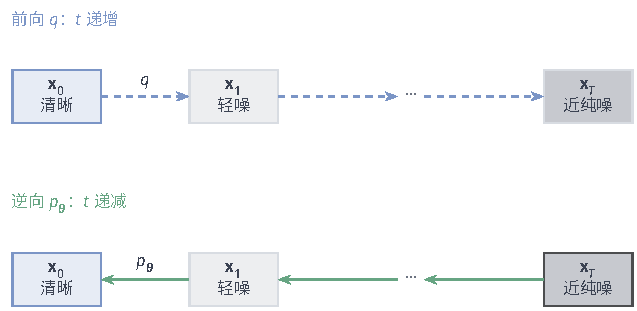
\includegraphics[width=\linewidth]{figures/03-models/03-probabilistic-graphical-models/tikz/pgm-generative-diffusion/figure.pdf}
  \caption{离散扩散的两条条件化链。上行是训练时固定的加噪过程，下行是从终端先验开始的生成过程；方框用逐渐加深的灰度和“清晰—轻噪—近纯噪”文字显示样本随$t$变化。相同下标表示相同噪声尺度，不表示两行抽样路径逐点相同；有限$T$时$q_T\approx p(\bm{x}_T)$需要日程与数据尺度支持。}
  \label{fig:pgm-generative-diffusion}
\end{figure}

图~\ref{fig:pgm-generative-diffusion}中的逆转移通常用神经网络参数化高斯均值及方差。这里有一个重要边界：对一般数据，真实$q(\bm{x}_{t-1}\mid\bm{x}_t)$是对未知$\bm{x}_0$混合后的分布，不保证为高斯。小步高斯逆转移是有限步模型的参数化选择；下面可解析的高斯是额外给定$\bm{x}_0$的$q(\bm{x}_{t-1}\mid\bm{x}_t,\bm{x}_0)$。二者不可混同。

图~\ref{fig:diffusion-sample-process-illustration}用样本插画补充两条链的读法。下行从独立的终端噪声开始，并不是把上行的一次随机加噪逐步撤销。

\begin{figure*}[htbp]
  \centering
  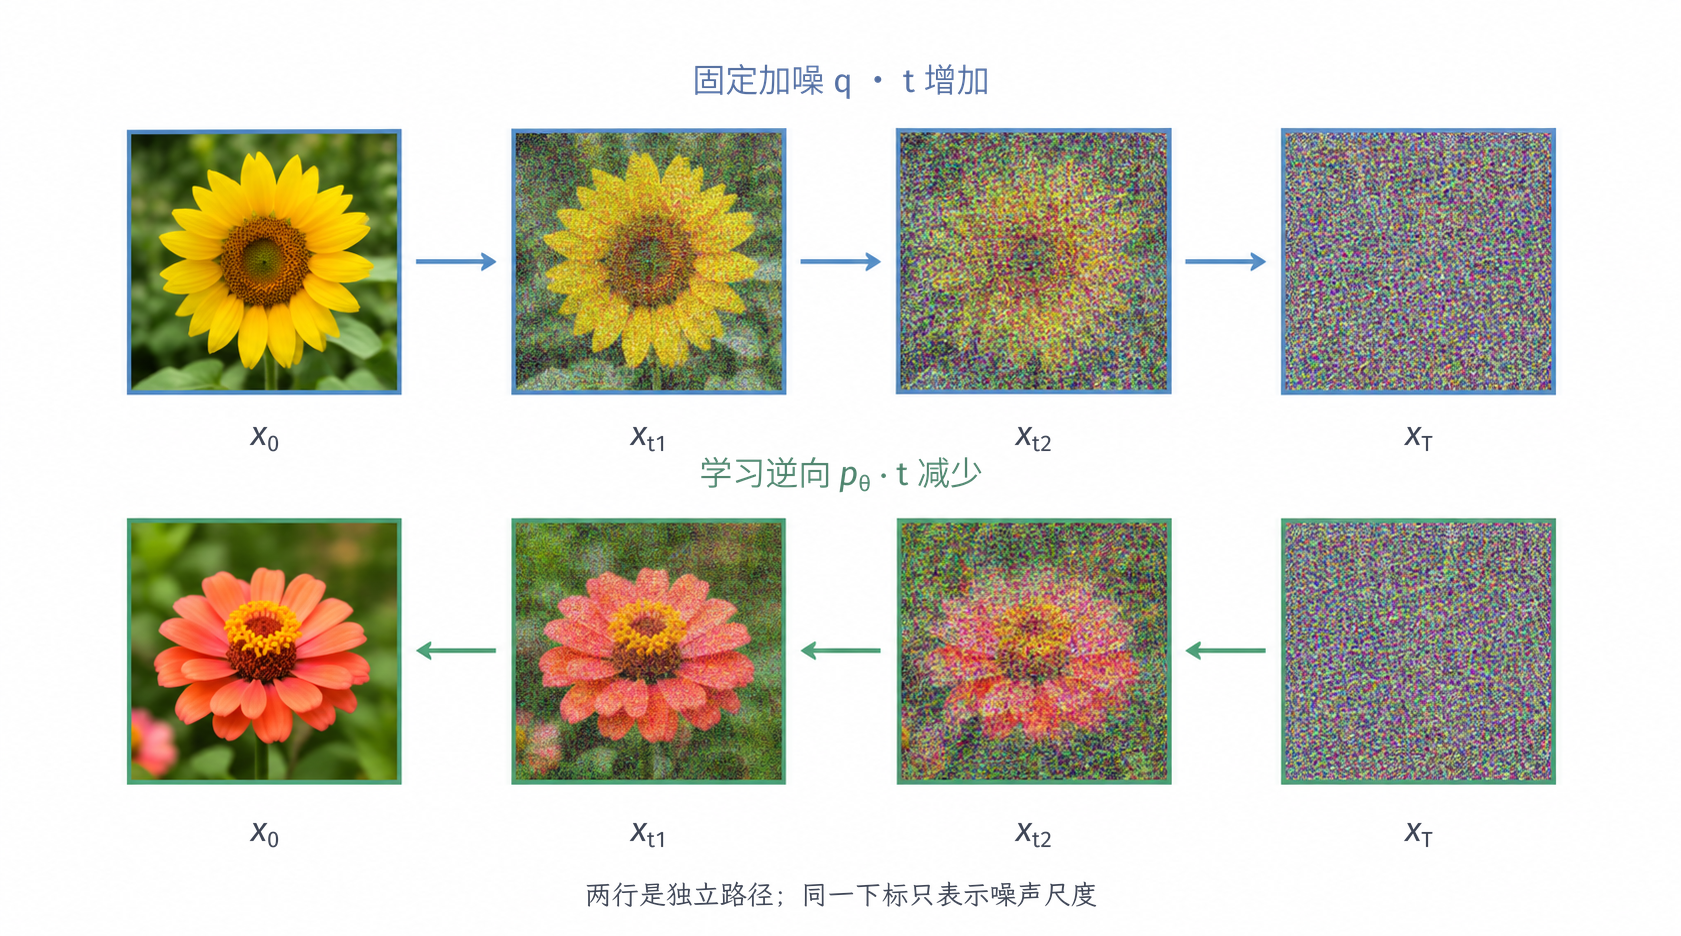
\includegraphics[width=\linewidth]{figures/03-models/03-probabilistic-graphical-models/generated/diffusion-sample-process-illustration/figure.png}
  \caption{离散扩散的样本变化示意。上行为固定的前向加噪，时间从左向右增加；下行为学习到的逆向生成，从右侧独立终端噪声开始，时间向左减少。相同下标只对应噪声尺度，两行不是同一次加噪与还原。花朵及中间样本为机制插画，不是数值加噪数据或一次真实模型实验。}
  \label{fig:diffusion-sample-process-illustration}
\end{figure*}

\subsection{变分目标与分数匹配}
\label{sec:pgm-generative-diffusion-objective}

为了学习式~\eqref{eq:pgm-generative-reverse-joint}，把整条$\bm{x}_{1:T}$路径视为潜变量，固定$\bm{x}_0$后应用式~\eqref{eq:pgm-variational-elbo}。这里的观测是$\bm{x}_0$，一般公式中的$\bm{z}$则由整条加噪路径代替。记$\mathcal{B}_{\mathrm{diff}}(\bm{x}_0)$为路径下界，负下界为$\mathcal{J}_{\mathrm{diff}}=-\mathcal{B}_{\mathrm{diff}}$，则
\begin{equation}
  \label{eq:pgm-generative-path-elbo}
  \begin{aligned}
    \log p_{\bm{\theta}}(\bm{x}_0)
      &\geq\mathcal{B}_{\mathrm{diff}}(\bm{x}_0),\\
    \mathcal{J}_{\mathrm{diff}}(\bm{x}_0)
      &=\mathbb{E}_{q(\bm{x}_{1:T}\mid\bm{x}_0)}
         \left[\log
           \frac{q(\bm{x}_{1:T}\mid\bm{x}_0)}
                {p_{\bm{\theta}}(\bm{x}_{0:T})}
         \right].
  \end{aligned}
\end{equation}
要把这个路径比值化为局部计算，使用$t\geq2$时的Bayes恒等式
\[
  q(\bm{x}_t\mid\bm{x}_{t-1})
  =q(\bm{x}_{t-1}\mid\bm{x}_t,\bm{x}_0)
     \frac{q(\bm{x}_t\mid\bm{x}_0)}
          {q(\bm{x}_{t-1}\mid\bm{x}_0)}.
\]
代入前向连乘，右侧的边缘比值逐项消去，留下$q(\bm{x}_T\mid\bm{x}_0)\prod_{t=2}^{T}q(\bm{x}_{t-1}\mid\bm{x}_t,\bm{x}_0)$。对每个$\bm{x}_{t-1}$先取条件期望，就得到
\begin{equation}
  \label{eq:pgm-generative-ddpm-kl}
  \begin{aligned}
    \mathcal{J}_{\mathrm{diff}}(\bm{x}_0)
      ={}&\operatorname{KL}\bigl(
          q(\bm{x}_T\mid\bm{x}_0)\,\|\,p(\bm{x}_T)\bigr)\\
       &+\sum_{t=2}^{T}
         \mathbb{E}_{q(\bm{x}_t\mid\bm{x}_0)}
          \operatorname{KL}\bigl(
           q(\bm{x}_{t-1}\mid\bm{x}_t,\bm{x}_0)
           \,\|\,p_{\bm{\theta}}(\bm{x}_{t-1}\mid\bm{x}_t)
                         \bigr)\\
       &-\mathbb{E}_{q(\bm{x}_1\mid\bm{x}_0)}
          \log p_{\bm{\theta}}(\bm{x}_0\mid\bm{x}_1).
  \end{aligned}
\end{equation}
三部分分别是终点匹配、逐步逆转移匹配和观测解码。固定日程与先验时，第一项对$\bm{\theta}$是常数，可以在求梯度时省略，却不能在报告似然界时删掉。最后一项不是$t=1$的普通高斯KL，因为给定$\bm{x}_0$时它已经是观测值，不是一个具有正方差的待积分变量。

中间KL之所以可计算，是因为前向过程给定$\bm{x}_0$后全为高斯。对$t\geq2$，将$q(\bm{x}_t\mid\bm{x}_{t-1})q(\bm{x}_{t-1}\mid\bm{x}_0)$中关于$\bm{x}_{t-1}$的平方项相加，其精度系数为
\[
  \frac{\alpha_t}{\beta_t}
    +\frac{1}{1-\bar{\alpha}_{t-1}}
  =\frac{1-\bar{\alpha}_t}
          {\beta_t(1-\bar{\alpha}_{t-1})}.
\]
线性项相应为$\sqrt{\alpha_t}\bm{x}_t/\beta_t+\sqrt{\bar{\alpha}_{t-1}}\bm{x}_0/(1-\bar{\alpha}_{t-1})$。乘上精度的倒数，便得
\begin{equation}
  \label{eq:pgm-generative-forward-posterior}
  \begin{aligned}
    q(\bm{x}_{t-1}\mid\bm{x}_t,\bm{x}_0)
      &=\mathcal{N}(\bm{x}_{t-1};
          \widetilde{\bm{\mu}}_t,\widetilde{\beta}_t\bm{I}_d),\\
    \widetilde{\beta}_t
      &=\frac{\beta_t(1-\bar{\alpha}_{t-1})}
              {1-\bar{\alpha}_t},\\
    \widetilde{\bm{\mu}}_t
      &=\frac{\sqrt{\bar{\alpha}_{t-1}}\beta_t}
               {1-\bar{\alpha}_t}\bm{x}_0
       +\frac{\sqrt{\alpha_t}(1-\bar{\alpha}_{t-1})}
               {1-\bar{\alpha}_t}\bm{x}_t.
  \end{aligned}
\end{equation}
学习时$\bm{x}_0$已知，所以它可以出现在监督目标里；生成时未知，模型均值只能依赖当前$\bm{x}_t$、噪声步$t$和允许使用的外部条件。

现固定逆方差$\sigma_t^2>0$，令$p_{\bm{\theta}}(\bm{x}_{t-1}\mid\bm{x}_t)=\mathcal{N}(\bm{\mu}_{\bm{\theta}}(\bm{x}_t,t),\sigma_t^2\bm{I}_d)$。高斯KL分为均值误差与方差误差：
\begin{equation}
  \label{eq:pgm-generative-gaussian-step-kl}
  \begin{aligned}
    \operatorname{KL}(q\,\|\,p_{\bm{\theta}})
      &=\frac{\lVert\widetilde{\bm{\mu}}_t
                    -\bm{\mu}_{\bm{\theta}}(\bm{x}_t,t)\rVert_2^2}
               {2\sigma_t^2}+C_t,\\
    C_t&=\frac{d}{2}
       \left(\frac{\widetilde{\beta}_t}{\sigma_t^2}
              -1+\log\frac{\sigma_t^2}{\widetilde{\beta}_t}\right).
  \end{aligned}
\end{equation}
固定$\sigma_t^2$时$C_t$不依赖参数。常用选择包括$\sigma_t^2=\beta_t$和$t\geq2$时的$\sigma_t^2=\widetilde{\beta}_t$。若学习逆方差，则均值误差的权重和方差项都要参与优化，不能把后者当成常数；若方差只依赖$\bm{x}_t$而没有待学习参数，方差项虽仍对参数不变，也不再是仅依赖$t$的常数。

利用式~\eqref{eq:pgm-generative-forward-marginal}把$\bm{x}_0$换成$\bm{x}_t$和噪声，后验均值也可写成
\[
  \widetilde{\bm{\mu}}_t
  =\frac{1}{\sqrt{\alpha_t}}
       \left(\bm{x}_t-
          \frac{\beta_t}{\sqrt{1-\bar{\alpha}_t}}\bm{\epsilon}\right).
\]
因此可以让网络预测合成噪声$\bm{\epsilon}_{\bm{\theta}}(\bm{x}_t,t)$，再定义
\begin{equation}
  \label{eq:pgm-generative-noise-parameterization}
  \bm{\mu}_{\bm{\theta}}(\bm{x}_t,t)
  =\frac{1}{\sqrt{\alpha_t}}
       \left(\bm{x}_t-
          \frac{\beta_t}{\sqrt{1-\bar{\alpha}_t}}
               \bm{\epsilon}_{\bm{\theta}}(\bm{x}_t,t)\right).
\end{equation}
两均值相减时$\bm{x}_t$项抵消。记$\ell_t(\bm{\theta})$为第$t$个中间KL的数据与扰动平均，并仍按式~\eqref{eq:pgm-generative-forward-marginal}抽取$\bm{x}_t$，则
\begin{equation}
  \label{eq:pgm-generative-weighted-denoising}
  \begin{aligned}
    \ell_t(\bm{\theta})
      &=w_t\,\mathbb{E}_{\bm{x}_0,\bm{\epsilon}}
         \lVert\bm{\epsilon}
          -\bm{\epsilon}_{\bm{\theta}}(\bm{x}_t,t)\rVert_2^2+C_t,\\
    w_t&=\frac{\beta_t^2}
              {2\sigma_t^2\alpha_t(1-\bar{\alpha}_t)},
          \qquad t=2,\ldots,T.
  \end{aligned}
\end{equation}
这才是固定逆方差、噪声参数化下的ELBO去噪权重。权重不是可随意丢弃的全局比例因子，因为它一般随$t$变化。

\begin{example}[核对一个扩散步的权重]
  \label{ex:pgm-generative-step-weight}
  为方便计算，人为取$\beta_1=0.2$、$\beta_2=0.25$，于是$\alpha_2=0.75$、$\bar{\alpha}_1=0.8$、$\bar{\alpha}_2=0.6$。在$t=2$时，$\widetilde{\beta}_2=0.25(0.2)/0.4=0.125$。若$\sigma_2^2=0.25$，则$w_2=0.25^2/(2\cdot0.25\cdot0.75\cdot0.4)=5/12$。一维噪声预测误差为$0.3$时，均值差的平方为
  \[
    \frac{0.25^2}{0.75\cdot0.4}(0.3)^2=0.01875,
  \]
  除以$2\sigma_2^2=0.5$得到$0.0375$，恰等于$(5/12)(0.3)^2$。完整KL还须加$C_2=\tfrac12(0.5-1+\log2)\approx0.09657$。这里的大噪声步只用于代数核验，不代表推荐训练日程。
\end{example}

DDPM常用的简化目标则去掉逐步权重。独立抽取$t\sim\operatorname{Unif}\{1,\ldots,T\}$、$\bm{x}_0\sim p_{\mathrm{data}}$和$\bm{\epsilon}\sim\mathcal{N}(\bm{0},\bm{I}_d)$，目标为
\begin{equation}
  \label{eq:pgm-generative-simple-loss}
  \mathcal{J}_{\mathrm{simple}}
  =\mathbb{E}_{t,\bm{x}_0,\bm{\epsilon}}
      \lVert\bm{\epsilon}
       -\bm{\epsilon}_{\bm{\theta}}(\bm{x}_t,t)\rVert_2^2.
\end{equation}
它去掉了式~\eqref{eq:pgm-generative-weighted-denoising}的逐步权重，并对$t=1$也使用噪声回归。因而其数值不是原始负ELBO，负值也不能直接作为对数似然下界报告。原始DDPM对离散像素采用量化区间积分作为解码质量，简化损失并不等于这个精确解码项；对连续数据使用固定方差高斯解码时，解码负对数似然可换成带特定权重的平方误差，但去掉权重依然改变目标\scite{pgm-generative-ho2020}

若要随机抽步但仍优化严格ELBO，可令$t\in\{2,\ldots,T\}$按概率$\pi_t>0$抽取，用$w_t\lVert\bm{\epsilon}-\bm{\epsilon}_{\bm{\theta}}\rVert_2^2/\pi_t$无偏估计中间项中依赖参数的部分，并单独处理解码项。均匀抽步时补上步数因子即可；若要报告完整界值，还须计入$C_t$及终点项。改变抽样概率并做重要性校正，改变的是估计方差；不做校正而改变步权重，改变的才是优化准则。对无限表达能力且各噪声尺度可独立拟合的理想模型，正权重不改变每步平方回归的最优条件均值；对共享有限网络，各步竞争同一组参数，权重会影响实际折中。

噪声回归还给出另一种解释。记$q_t(\bm{x})$为前向扰动后的边缘密度，其\term{分数}（score）是$\bm{s}_t^*(\bm{x})=\nabla_{\bm{x}}\log q_t(\bm{x})$，表示密度沿各坐标增加的局部方向，而不是分类分数。为与前向路径$q$保持一致，本章写$q_t$；许多分数模型文献把同一个前向边缘记作$p_t$。高斯扰动的条件分数已知：
\[
  \nabla_{\bm{x}_t}\log q(\bm{x}_t\mid\bm{x}_0)
  =-\frac{\bm{x}_t-\sqrt{\bar{\alpha}_t}\bm{x}_0}
           {1-\bar{\alpha}_t}
  =-\frac{\bm{\epsilon}}{\sqrt{1-\bar{\alpha}_t}}.
\]
若可以交换微分与积分，对$q_t(\bm{x}_t)=\int q(\bm{x}_t\mid\bm{x}_0)p_{\mathrm{data}}(\bm{x}_0)\,\mathrm{d}\bm{x}_0$求导并除以$q_t(\bm{x}_t)>0$，得到
\begin{equation}
  \label{eq:pgm-generative-denoising-identity}
  \bm{s}_t^*(\bm{x}_t)
  =\mathbb{E}\!\left[
       \nabla_{\bm{x}_t}\log q(\bm{x}_t\mid\bm{X}_0)
       \mid\bm{x}_t\right]
  =-\frac{\mathbb{E}[\bm{\epsilon}\mid\bm{x}_t]}
            {\sqrt{1-\bar{\alpha}_t}}.
\end{equation}
平方回归的最优预测就是条件均值，因而令$\bm{s}_{\bm{\theta}}=-\bm{\epsilon}_{\bm{\theta}}/\sqrt{1-\bar{\alpha}_t}$，噪声回归便在估计各尺度的边缘分数，并不是恢复每个样本唯一的“真实噪声”。

\term{去噪分数匹配}（denoising score matching, DSM）用已知扰动核的条件分数作为训练目标，学习未知边缘分数。更精确地，令$\bm{a}=\nabla_{\bm{x}_t}\log q(\bm{x}_t\mid\bm{X}_0)$，由条件期望的正交分解，在平方矩有限时
\begin{equation}
  \label{eq:pgm-generative-dsm-decomposition}
  \mathbb{E}\lVert\bm{s}_{\bm{\theta}}-\bm{a}\rVert_2^2
  =\mathbb{E}\lVert\bm{s}_{\bm{\theta}}-\bm{s}_t^*\rVert_2^2
   +\mathbb{E}\lVert\bm{a}-\bm{s}_t^*\rVert_2^2.
\end{equation}
最后一项与网络无关，这给出了去噪训练能够学习边缘分数的依据。对于当前高斯核，噪声平方误差等于$(1-\bar{\alpha}_t)$乘以条件分数平方误差。因此简化噪声损失对应一种DSM尺度加权，严格ELBO对应另一种加权；任意正权重DSM不自动成为同一个生成模型的ELBO。连续时间分数建模将这些噪声尺度连成一个共同框架\scite{pgm-generative-song2021}

把式~\eqref{eq:pgm-generative-noise-parameterization}改用分数表示，还得到
\[
  \bm{\mu}_{\bm{\theta}}(\bm{x}_t,t)
    =\frac{\bm{x}_t+\beta_t\bm{s}_{\bm{\theta}}(\bm{x}_t,t)}
            {\sqrt{\alpha_t}}.
\]
若分数精确，它给出真实逆转移的条件均值，但没有证明逆转移整体为高斯。在式~\eqref{eq:pgm-generative-gaussian-diffusion}的例子中，$\bm{s}_t^*$的一维形式为$-x_t/(1+4\bar{\alpha}_t)$，所以读者可直接把它代入检验均值。与第~\ref{chap:pgm-energy-models}章相连，若$q_t(\bm{x})\propto\exp[-E_t(\bm{x})]$，则$\bm{s}_t^*=-\nabla E_t$，归一化常数在求导后消失。但一般向量网络不必恰好是某个标量能量的梯度；给出分数近似，不等于已经提供可直接评价的归一化密度。

算法~\ref{alg:pgm-generative-ddpm}给出一个具体的连续观测版本：所有$\sigma_t^2>0$都预先固定，均值均由式~\eqref{eq:pgm-generative-noise-parameterization}给出，包括$t=1$的高斯解码分布$p_{\bm{\theta}}(\bm{x}_0\mid\bm{x}_1)$。因此解码器没有独立于噪声网络、却又未被损失训练的参数。

\begin{algorithm}[固定方差DDPM的学习与祖先采样]
  \label{alg:pgm-generative-ddpm}
  \begin{algorithmic}[1]
    \Require 连续观测数据集、固定$\beta_{1:T}$及正的逆转移方差$\sigma_{1:T}^2$
    \Ensure 学得的噪声网络与模型样本
    \State 初始化$\bm{\theta}$，预计算$\alpha_t,\bar{\alpha}_t$
    \For{每个训练小批量，直至停止条件满足}
      \State 为每个观测抽$t\sim\operatorname{Unif}\{1,\ldots,T\}$和标准高斯$\bm{\epsilon}$
      \State 按式~\eqref{eq:pgm-generative-forward-marginal}计算$\bm{x}_t$
      \State 由式~\eqref{eq:pgm-generative-simple-loss}更新参数
    \EndFor
    \State 抽$\bm{x}_T\sim\mathcal{N}(\bm{0},\bm{I}_d)$
    \For{$t=T,T-1,\ldots,2$}
      \State 用噪声网络和式~\eqref{eq:pgm-generative-noise-parameterization}计算$\bm{\mu}_{\bm{\theta}}$
      \State 独立抽$\bm{\xi}_t\sim\mathcal{N}(\bm{0},\bm{I}_d)$，令$\bm{x}_{t-1}=\bm{\mu}_{\bm{\theta}}+\sigma_t\bm{\xi}_t$
    \EndFor
    \State 抽$\bm{x}_0\sim p_{\bm{\theta}}(\bm{x}_0\mid\bm{x}_1)$并返回
  \end{algorithmic}
\end{algorithm}

算法~\ref{alg:pgm-generative-ddpm}明确使用简化训练损失；若目标是严格变分学习，应替换相应训练步骤并保留解码项。对连续高斯解码，$\sigma_1^2$须单独取正值，不能把$\widetilde{\beta}_1=0$代入非退化高斯密度。有些生成程序在最后一步直接输出预测均值，这是一种确定性末步约定，并非对正方差解码分布的完整采样。若一次网络前向代价为$C_{\mathrm{net}}$，抽步训练的单样本前向代价约为$O(C_{\mathrm{net}}+d)$，而完整$T$步祖先采样约为$O(T(C_{\mathrm{net}}+d))$。采样只需保留当前状态，不必保存整条路径；若要评价全路径变分界，则还需处理所有项或使用带校正的随机估计。

\subsection{连续时间表示与采样}
\label{sec:pgm-generative-continuous-diffusion}

当噪声步变得足够细，可以把人工噪声索引写成连续$t\in[0,T_{\mathrm{c}}]$，其中$T_{\mathrm{c}}$为连续过程的终点。为避免隐藏额外导数项，下面只讨论扩散系数依赖$t$、不依赖状态的各向同性情形。设$\bm{W}_t$为$d$维标准\term{布朗运动}（Brownian motion）：不相交时间区间上的增量相互独立，长度为$\Delta t$的增量服从$\mathcal{N}(\bm{0},\Delta t\,\bm{I}_d)$。前向\term{随机微分方程}（stochastic differential equation, SDE）为
\begin{equation}
  \label{eq:pgm-generative-forward-sde}
  \mathrm{d}\bm{X}_t
  =\bm{b}(\bm{X}_t,t)\,\mathrm{d}t
    +g(t)\,\mathrm{d}\bm{W}_t,
  \qquad \bm{X}_0\sim p_{\mathrm{data}}.
\end{equation}
其中漂移$\bm{b}$规定确定性的局部移动，$g(t)>0$规定噪声强度。本节假设系数连续，$\bm{b}$对空间全局Lipschitz且至多线性增长，$g$有界并在所讨论的闭区间上有正下界，以保证前向解存在且不爆炸。使用反向密度公式时，进一步假设$q_t>0$，对时间一阶、对空间二阶连续可微，在所用时间区间上$\int\mathbb{E}_{q_t}\lVert\nabla\log q_t(\bm{X}_t)\rVert_2^2\,\mathrm{d}t<\infty$，并且反向方程存在不爆炸的解。若数据本身奇异，这些密度条件可以只在$t\geq\delta>0$的已加噪区间成立，不能默认$t=0$也有光滑密度。

与离散DDPM对应的方差保持过程取$\bm{b}(\bm{x},t)=-\tfrac12\beta(t)\bm{x}$、$g(t)=\sqrt{\beta(t)}$。其条件均值衰减系数为$\exp[-\tfrac12\int_0^t\beta(s)\,\mathrm{d}s]$，条件方差为$1-\exp[-\int_0^t\beta(s)\,\mathrm{d}s]$。因此只要有限$T_{\mathrm{c}}$内积分有限，终点一般仍只是接近标准高斯；连续时间本身没有消除终点近似。

在这种条件扰动核可解析的设定中，训练可以从连续区间抽取$t$，构造$\bm{x}_t$，再拟合条件分数$\nabla_{\bm{x}_t}\log q(\bm{x}_t\mid\bm{x}_0)$。式~\eqref{eq:pgm-generative-denoising-identity}与式~\eqref{eq:pgm-generative-dsm-decomposition}对每个$t>0$仍然适用。时间抽样密度与损失权重共同决定各噪声尺度的训练比重；这仍是去噪分数学习，不能仅因把时间变成连续就将其数值解释为观测似然。

记真分数为$\bm{s}_t^*=\nabla_{\bm{x}}\log q_t$。在上述正则条件及反向过程存在的设定下，反向SDE可以沿同一个$t$写成
\begin{equation}
  \label{eq:pgm-generative-reverse-sde}
  \begin{aligned}
    \mathrm{d}\bm{X}_t
    ={}&\bigl[\bm{b}(\bm{X}_t,t)-g(t)^2\bm{s}_t^*(\bm{X}_t)\bigr]
         \,\mathrm{d}t\\
       &+g(t)\,\mathrm{d}\overline{\bm{W}}_t,
    \qquad t:T_{\mathrm{c}}\downarrow0.
  \end{aligned}
\end{equation}
这里$\mathrm{d}t<0$，反向布朗增量的协方差是$|\mathrm{d}t|\bm{I}_d$。不能把括号里的漂移原样拿去按正时间步长运行。为消除实现上的符号歧义，令$u=T_{\mathrm{c}}-t$、$\bm{Y}_u=\bm{X}_{T_{\mathrm{c}}-u}$，则按递增$u$运行的等价形式是
\begin{equation}
  \label{eq:pgm-generative-positive-reverse-time}
  \begin{aligned}
    \mathrm{d}\bm{Y}_u
      ={}&-\bm{b}(\bm{Y}_u,T_{\mathrm{c}}-u)\,\mathrm{d}u\\
         &+g(T_{\mathrm{c}}-u)^2
              \bm{s}_{T_{\mathrm{c}}-u}^*(\bm{Y}_u)\,\mathrm{d}u\\
         &+g(T_{\mathrm{c}}-u)\,\mathrm{d}\bm{B}_u.
  \end{aligned}
\end{equation}
其中$\bm{B}_u$是按递增$u$定义的标准布朗运动。这是真分数下的时间反演结果；其一般证明需要随机过程的反演理论，这里采用已有结果，不把仅验证边缘方程充作路径反演的完整证明。分数SDE框架给出了该公式及更一般的状态相关扩散版本；后一种情形还会出现扩散矩阵的空间导数，不能直接照搬本式\scite{pgm-generative-song2021}

式~\eqref{eq:pgm-generative-positive-reverse-time}也给出明确的数值一步。令$t=T_{\mathrm{c}}-u$、$\Delta u>0$，用学得分数替代真分数的Euler--Maruyama更新为
\[
  \begin{aligned}
    \bm{y}_{u+\Delta u}
      ={}&\bm{y}_u-\bm{b}(\bm{y}_u,t)\Delta u\\
         &+g(t)^2\bm{s}_{\bm{\theta}}(\bm{y}_u,t)\Delta u
          +g(t)\sqrt{\Delta u}\,\bm{\xi},
  \end{aligned}
\]
其中$\bm{\xi}\sim\mathcal{N}(\bm{0},\bm{I}_d)$，每步独立抽取。漂移中的分数项为正号，使用真分数时该项沿密度增加的方向移动；这个正号与式~\eqref{eq:pgm-generative-reverse-sde}中的负号并不矛盾，两式使用的时间方向不同。要精确恢复前向数据分布，还必须从真实$q_{T_{\mathrm{c}}}$启动并精确求解；换成简单终端先验、估计分数和离散求解都会引入各自的误差。

是否每次采样都必须在途中加入随机噪声？在真分数可得的理想条件下，可以构造与前向SDE具有相同各时刻边缘密度的确定性方程。\term{概率流常微分方程}（probability flow ordinary differential equation, probability flow ODE）定义速度
\begin{equation}
  \label{eq:pgm-generative-probability-flow}
  \frac{\mathrm{d}\bm{X}_t}{\mathrm{d}t}
     =\bm{v}^*(\bm{X}_t,t),
  \qquad
  \bm{v}^*(\bm{x},t)
     =\bm{b}(\bm{x},t)-\frac12g(t)^2\bm{s}_t^*(\bm{x}).
\end{equation}
它不是简单地删除逆SDE的噪声项，分数系数还必须从$1$改成$1/2$。给定终点后，ODE轨迹确定；不同样本的随机性来自不同的终点抽样。

这个系数可以由密度守恒推导。前向SDE的Fokker--Planck方程为
\[
  \partial_t q_t
    =-\nabla\cdot(\bm{b}q_t)+\tfrac12g(t)^2\Delta q_t.
\]
利用$q_t\bm{s}_t^*=\nabla q_t$以及$g$不依赖$\bm{x}$，右侧等于
\[
  -\nabla\cdot
       \left[\left(\bm{b}-\tfrac12g(t)^2\bm{s}_t^*\right)q_t\right],
\]
这正是速度场$\bm{v}^*$的连续性方程。在适当边界衰减、共同初始密度及密度方程唯一性条件下，ODE与SDE具有相同的单时刻边缘。这个推导没有声称它们的多时刻联合分布或单条轨迹相同：随机扩散路径与确定性流路径本来就是不同的对象。

令$\bm{v}_{\bm{\theta}}=\bm{b}-\tfrac12g^2\bm{s}_{\bm{\theta}}$，并给ODE指定可评价密度的终端先验$p_{T_{\mathrm{c}}}$。若这一速度场生成正反均存在的可微流，便独立定义了一个ODE密度模型$p_{\bm{\theta}}^{\mathrm{ODE}}$。将式~\eqref{eq:pgm-generative-instantaneous-change}沿数据到终点的方向积分，得到
\begin{equation}
  \label{eq:pgm-generative-ode-likelihood}
  \begin{aligned}
    \log p_{\bm{\theta}}^{\mathrm{ODE}}(\bm{x}_0)
       &=\log p_{T_{\mathrm{c}}}(\bm{x}_{T_{\mathrm{c}}})
          +\int_0^{T_{\mathrm{c}}}
            \nabla_{\bm{x}}\cdot
            \bm{v}_{\bm{\theta}}(\bm{x}_t,t)\,\mathrm{d}t,\\
    \frac{\mathrm{d}\bm{x}_t}{\mathrm{d}t}
       &=\bm{v}_{\bm{\theta}}(\bm{x}_t,t),
       \qquad \bm{x}_{t=0}=\bm{x}_0.
  \end{aligned}
\end{equation}
积分前面是正号，因为瞬时公式给出的是终点对数密度减去起点对数密度等于负散度积分，现在求解的是起点密度。评价似然时从数据向噪声积分，生成时从终端向数据积分；二者使用同一速度场和相反的积分方向。

例如一维速度$v(x,t)=ax$、$T_{\mathrm{c}}=1$、终端密度$\mathcal{N}(0,1)$时，$x_1=e^a x_0$，散度积分为$a$，所以
\[
  \log p^{\mathrm{ODE}}(x_0)
  =-\tfrac12\log(2\pi)-\tfrac12e^{2a}x_0^2+a.
\]
这恰是$\mathcal{N}(0,e^{-2a})$的对数密度。取$a=-\tfrac12\log5$，又得到贯穿例子的$\mathcal{N}(0,5)$；若把式~\eqref{eq:pgm-generative-ode-likelihood}的积分符号写反，归一化因子就会出错。这个线性场仅用来核对变量变换，不假定它就是前述方差保持SDE的概率流。

“ODE可以计算似然”必须带上模型对象和数值条件。近似分数代入ODE后，式~\eqref{eq:pgm-generative-ode-likelihood}仍是该ODE所定义分布的密度公式，但一般不等于使用同一近似分数的随机SDE分布，更不自动等于某个有限步DDPM的边缘似然。真分数、正确终点与精确积分时的同边缘结论，不能无条件转移给三个近似实现。

数值评价还需要沿轨迹计算散度。使用随机向量估计$\nabla\cdot\bm{v}_{\bm{\theta}}$时会有蒙特卡洛误差；有限容差的ODE求解器会产生轨迹与积分误差，二者的数值耦合也不能用迹估计无偏一句话消除。若只积分到$\delta>0$，得到的是该截断模型在$\delta$处的密度，还需说明从$\delta$到观测空间的解码或近似。对离散像素报告似然，另须统一去量化与测度约定。改善求解器容差不能修复分数偏差，增加迹样本也不能消除终点先验失配。

采样速度应以网络函数评价次数而非仅以“步数”衡量。一个高阶ODE步骤可能多次调用网络；自适应求解器还可能拒绝某次试步。随机采样允许每步注入噪声，确定性采样便于固定终点后的重复生成和编码，但在近似网络与有限预算下，二者不存在脱离设定的质量排序。减少离散步数通常降低计算，却改变数值误差；若原本讨论的就是有限步DDPM，完整执行其每个转移是从该离散模型采样，跳过转移则定义了另一套采样近似。

\term{采样蒸馏}（sampling distillation）进一步用一个已训练采样器的多步输出监督另一个少步模型。渐进蒸馏可把两个确定性教师步骤压成一个学生步骤，重复这一过程降低生成时的函数评价次数\scite{pgm-generative-salimans2022}

代价转移到额外训练及学生对教师的近似中；学生映射若没有相应的可逆性和密度追踪机制，也不会自动继承教师ODE的似然公式。无论采用求解器加速还是蒸馏，扩散索引始终是人为噪声尺度。对视频等真实时序数据，可以在整个序列或其潜表示上另加一条扩散轴，但必须把这两个索引分开。

\section{模型关系与比较}
\label{sec:pgm-generative-comparison}

\subsection{似然、后验与采样}
\label{sec:pgm-generative-likelihood-posterior-sampling}

比较这些模型时，应固定查询对象。完整观测的密度、给定部分观测的条件分布、潜变量后验、无条件样本是四种不同查询。Flow完整密度可算，并不意味着对任意缺失坐标的积分也可算；VAE有快速编码器，并不意味着它输出了精确后验；DDPM能随机抽步训练，也不意味着生成只需一步。

VAE、Flow和扩散并未用尽换取可计算性的办法。\term{概率电路}（probabilistic circuit, PC）把分布写成由简单叶分布、加权和节点及乘积节点构成的计算图。叶节点能精确评价和边缘化；和节点执行混合，乘积节点组合不同变量块。它以结构约束控制计算，而不是要求每个高维变换可逆\scite{pgm-generative-choi2020}

一种足够的归一化设定是：每个叶分布归一化，和节点权重非负且和为$1$；和节点各孩子涉及同一组变量，称为\term{光滑性}（smoothness），也称完备性；乘积节点各孩子涉及互不相交的变量组，称为\term{可分解性}（decomposability）。由叶向根归纳，和保持归一化，互不相交变量上的乘积也保持归一化。边缘化时可在叶节点上先积分，再沿相同加法和乘法向上传播，因为可分解性允许把对不同变量块的积分拆开。设边数为$m$且叶查询为常数成本，则一次向上传播为$O(m)$；条件化分母的边缘概率质量或密度为正时，条件分布可由两个相应边缘量之比得到。

这类结论是相对于已经给定的电路大小而言的，某些分布可能需要很大的电路。上述条件也不保证所有MAP或边缘MAP查询都同样容易，不能把求和直接换成最大化便宣称解决。对本章的比较而言，概率电路补充了一个坐标：让完整密度可算与让大量边缘查询可算，是不同层次的结构要求。表~\ref{tab:pgm-generative-model-comparison}按这些计算对象概括本章的取舍。

\begin{table*}[htbp]
  \centering
  \small
  \begin{tabularx}{\linewidth}{@{}lXXX@{}}
    \toprule
    机制 & 完整观测的似然 & 潜变量与条件查询 & 典型采样代价与限制 \\
    \midrule
    自回归基线
      & 条件分解给出精确似然
      & 一般缺失坐标不一定能高效边缘化
      & 通常按坐标顺序生成；依赖排序 \\
    VAE
      & 通常优化ELBO，边缘似然需额外估计
      & 编码器给出近似后验
      & 先抽潜变量再解码；条件似然决定额外成本 \\
    离散层Flow
      & 逆变换与Jacobian可行时精确
      & 完整观测有唯一逆像；部分观测仍可能需积分
      & 逐层变换；自回归流有方向性成本 \\
    DDPM
      & 路径ELBO可估计；简化损失不是似然值
      & 固定前向路径充当变分分布
      & 多步随机转移；有限终点与参数化有误差 \\
    分数ODE
      & 散度积分定义ODE模型密度
      & 可逆流给出编码，不是随机路径后验
      & 数值积分；精度与函数评价次数相关 \\
    受约束概率电路
      & 可精确评价归一化密度或质量
      & 合适结构下可精确边缘化与条件查询
      & 结构化采样；表示规模可能很大 \\
    \bottomrule
  \end{tabularx}
  \caption{统一查询口径下的比较。“精确”指模型中无需变分或边缘化近似的数学计算关系，不排除浮点误差；连续流和分数ODE还涉及数值积分及可能的随机迹估计。概率电路一行采用正文给出的光滑、可分解及归一化条件。}
  \label{tab:pgm-generative-model-comparison}
\end{table*}

即使似然评价完全一致，生成质量也没有因此被一个数值穷尽。似然比较必须使用相同观测表示、测度和预处理；样本是否具有任务所需结构、是否覆盖多种模式、采样资源是否可接受，则需要各自的评价。贯穿例子中三条路线都可表达$\mathcal{N}(0,5)$，已经说明仅由边缘分布不能反推出唯一的计算机制或潜变量解释。复杂数据上，有限网络容量、推断族与数值预算会把这些机制上的差异转化为实际误差。

\subsection{生成机制的组合}
\label{sec:pgm-generative-hybrids}

三种机制的组合应从“哪一个分布被改变”判断。Flow后验只把$q_{\bm{\phi}}(\bm{z}\mid\bm{x})$变得灵活，主要针对近似族误差；若基础后验和新增变换允许保留原分布作为特例，理论最优下界不会因扩族而降低，但实际优化不保证达到它。给VAE换成Flow先验，则改变了$p_{\bm{\theta}}(\bm{z})$，直接作用于生成时如何访问潜空间。两者都出现可逆网络，却解决不同的问题。

层次VAE把复杂性放进多层随机依赖。对于前文的两层例子，若取$q_{\bm{\phi}}(\bm{z}_1,\bm{z}_2\mid\bm{x})=q_{\bm{\phi}}(\bm{z}_1\mid\bm{x})q_{\bm{\phi}}(\bm{z}_2\mid\bm{z}_1,\bm{x})$，ELBO就是
\[
  \mathbb{E}_{q_{\bm{\phi}}}
  \left[
    \log\frac{
      p(\bm{z}_2)p_{\bm{\theta}}(\bm{z}_1\mid\bm{z}_2)
          p_{\bm{\theta}}(\bm{x}\mid\bm{z}_1)}
      {q_{\bm{\phi}}(\bm{z}_1\mid\bm{x})
          q_{\bm{\phi}}(\bm{z}_2\mid\bm{z}_1,\bm{x})}
  \right].
\]
它仍是同一个联合与变分路径之比。逐层抽样可以估计该期望，但每层都有自己的后验匹配问题；增加层数不自动消除坍塌。扩散也含多层潜状态，但其尺度、固定前向核及局部目标具有专门设计，不能仅因为“层数多”就与任意层次VAE等同。

\term{潜空间扩散}（latent diffusion）把多步生成放在观测的潜表示中：先学习编码与解码，再在编码得到的潜变量分布上训练扩散模型，最后把生成的潜变量解码为观测。其主要计算收益来自反复去噪的空间更小；原始潜空间扩散工作在预训练自编码表示上构造这一过程\scite{pgm-generative-rombach2022}

若解码器是归一化条件分布$p_{\bm{\psi}}(\bm{x}\mid\bm{z})$，潜空间生成先验为$p_{\bm{\theta}}^{\mathrm{diff}}(\bm{z})$，整体模型为
\begin{equation}
  \label{eq:pgm-generative-latent-diffusion}
  p_{\bm{\theta},\bm{\psi}}(\bm{x})
  =\int p_{\bm{\psi}}(\bm{x}\mid\bm{z})
          p_{\bm{\theta}}^{\mathrm{diff}}(\bm{z})\,\mathrm{d}\bm{z}.
\end{equation}
这又回到了潜变量边缘化：即使潜空间密度可评价，也不能省略观测空间的积分。若解码器只是非可逆确定性网络，或编码阶段主要用感知损失训练，就不能自动宣称得到了同一像素空间上的可计算似然。压缩误差、潜空间分布拟合和解码条件分布的局限，都需要分别考察。这些组合把计算放到了更合适的位置，但没有免除每一层概率定义的责任。

\subsection{与隐式生成模型的边界}
\label{sec:pgm-generative-implicit-boundary}

假设只给出$\bm{Z}\sim p_0$和生成程序$\bm{X}=G_{\bm{\theta}}(\bm{Z})$。对任意可测集合$B$，它已经规定
\begin{equation}
  \label{eq:pgm-generative-pushforward}
  \mathbb{P}_{\bm{\theta}}(\bm{X}\in B)
  =\int \mathbf{1}\{G_{\bm{\theta}}(\bm{z})\in B\}
           p_0(\bm{z})\,\mathrm{d}\bm{z}.
\end{equation}
这种通过采样程序间接规定的分布称为\term{隐式分布}（implicit distribution）。\term{生成对抗网络}（generative adversarial network, GAN）是常见例子：通常的生成器提供样本，却不提供像式~\eqref{eq:pgm-generative-flow-density}那样可直接评价的观测密度。本节只比较这一概率语义，不展开其对抗训练过程\scite{pgm-generative-goodfellow2014}

困难既可能是计算性的，也可能是测度上的。同维光滑映射即使处处局部可逆，只要全局多对一，密度通常也要累加所有逆像的贡献；普通网络没有保证逆像可枚举。若$\bm{Z}$维度小于观测维度，且$G_{\bm{\theta}}$为通常的局部Lipschitz网络，输出还可能集中在低维集合上，不具有相对于整个观测空间Lebesgue测度的密度。它仍是合法概率分布，只是不适用本章默认的$d$维密度公式。

Flow也把噪声推送成观测，所以“由噪声生成”不是GAN与Flow的边界。边界在于是否额外规定可逆性、同维变换、可计算体积因子等条件，使隐含分布具有可评价密度。VAE与离散扩散的观测密度虽然通常难以直接求值，但它们给出可评价的联合分布和明确的边缘化对象，因而能构造有概率含义的似然下界。能够采样、存在密度、密度可算、能算似然界，是针对不同性质和计算任务的陈述；不能从能够采样直接推出其余几项，也不能用一个下界代替密度本身。

\section{本章小结}
\label{sec:pgm-generative-summary}

复杂生成模型的共同难题不是单纯增加网络容量，而是在归一化、密度评价、推断和采样之间安排可计算的结构。VAE允许多个潜变量解释同一观测，以边缘化定义密度，用近似后验和ELBO支撑学习；规范化流用同维可逆变换让每个完整观测有唯一逆像，以Jacobian追踪体积；扩散把生成放在人工噪声过程上，用可计算的局部去噪问题学习逆转移。这三种机制可以组合，也可以表达相同的观测分布，却具有不同的潜变量含义和查询成本。

比较训练目标时，需要保留被简化的部分。VAE的重构项由观测似然决定，灵活后验不自动使观测似然精确可算；DDPM的严格路径ELBO包含终点项、逐步加权KL和解码项，均匀噪声回归不是其数值替身。连续时间下，逆SDE的符号必须与递减时间一起理解，概率流ODE的同边缘结论需要真分数和匹配的边界条件；计算ODE模型似然还需散度积分，并承担数值与迹估计误差。

模型选择因此应从所需查询出发：需要快速潜变量推断，就考察近似后验及其误差；需要完整观测密度，就考察逆变换或积分成本；需要大量缺失变量查询，还要考察边缘化结构；需要低延迟生成，则应把每次网络评价和顺序依赖算入预算。显式联合分布、可评价密度和方便的采样程序并不是同一件事。明确这些区别，才能把生成样本的直观表现与模型实际支持的概率结论联系起来。
